
\section{层流扩散火焰}

\subsection{概述}
\subsection{无反应的恒定密度层流射流}
\subsubsection{物理描述}
无限大的容器里面充满着静止的流体(氧化剂),一股无反应的流体(燃料)喷入。

\textbf{气流核心}: 黏性力和扩散还不起作用,流体的速度和射流流体的质量分数保持不变,等于喷嘴出口的值。{\tiny 如果这个情况在管内流动那就完全不同了,根据质量守恒,显然它会加速。}

\begin{figure}[H]
    \centering
    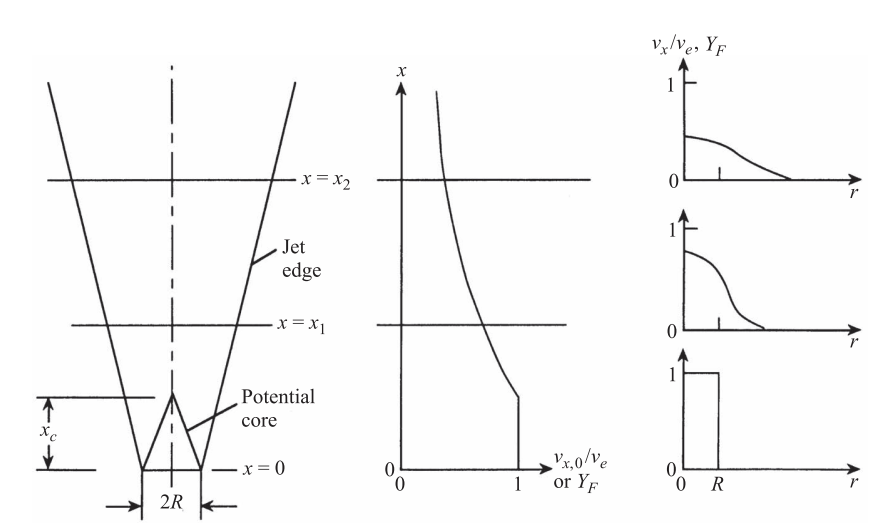
\includegraphics[width=.3\textwidth]{img/laminar_jet.png}
\end{figure}

显然存在着两个守恒:动量守恒和质量守恒,
\begin{eqnarray}
    2\pi\int_0^\infty \rho(r,x)v_x^2(r,x)r\dd r &=& \rho_e v_e^2\pi R^2\\
    2\pi\int_0^\infty \rho(r,x)v_x(r,x)Y_F(r,x)r\dd r &=& \rho_e v_e \pi R^2 Y_{F,e}
\end{eqnarray}

\subsubsection{假设}
\begin{enumerate}
    \item 射流和周围流体的摩尔质量相等。基于理想气体的性质,可以认为压力和温度都是常数,即整个流场内流体的密度为常数。
    \item 菲克扩散定律的简单二元扩散。
    \item 动量和组份扩散率为常数且相等等于1,施密特数(\(Sc\equiv \nu/\mathcal{D}\)等于1。
    \item 只考虑径向的动量和组分扩散,忽略轴向扩散。由于出口处轴向扩散很重要,所以下面的分析不适用于那里。
\end{enumerate}

\subsubsection{守恒定律}

\begin{equation}
    \begin{aligned}
        &\text{Mass:}&\frac{\pp v_x}{\pp x}+\frac{1}{r}\frac{\pp(v,r)}{\pp r}&=0\\
        &\text{Axial momentum:}& v_x \frac{\pp v_x}{\pp x}+ v_r\frac{\pp v_x}{\pp r} &= v\frac{1}{r}\frac{\pp}{\pp r}\left(r\frac{\pp v_x}{\pp r}\right)\\
        &\text{Species:}& v_x \frac{\pp Y_F}{\pp x} + v_r \frac{\pp Y_F}{\pp r}&=\mathcal{D}\frac{1}{r}\frac{\pp}{\pp r}\left(r\frac{\pp Y_F}{\pp r}\right)
    \end{aligned}
\end{equation}

那么对于氧化剂,有:
\begin{equation}
    Y_{Ox} = 1-Y_F
\end{equation}

\subsubsection{边界条件}
\begin{enumerate}
    \item 中心线的径向速度为0;
    \[v_r(0, x)=0\]
    \item 中心线的轴向速度在水平方向上变化率为0;
    \[\frac{\pp v_x}{\pp r}(0, x)=0\]
    \item 中心线的燃料质量分数在水平方向上变化率为0;
    \[\frac{\pp Y_F}{\pp r}(0, x)=0\]
    \item 轴向速度在径向的无穷远处为0;
    \[v_x(\infty, x)=0\]
    \item 燃料质量分数在径向无穷远处为0;
    \[Y_F(\infty, x) = 0\]
    \item 在出口处,速度和燃料质量分数都均匀且相等,出口外侧都为0;
    \[
        \begin{aligned}
            v_x(r\le R, 0) &=& v_e, \\
            v_x(r>R, 0) &=&0,\\
            Y_F(r\le R, 0)&=& Y_{F,e} = 1,\\
            Y_F(r>R, 0)&=&0.
        \end{aligned}
    \]
\end{enumerate}

\subsubsection{求解}
利用相似理论来进行求解,定义包含了\(r/x\)的相似变量\(\xi\)为:
\begin{equation}
    \xi = \left(\frac{3\rho_e J_e}{16\pi}\right)^{1/2}\frac{1}{\mu}\frac{r}{x}
\end{equation}

再定义初始流体动量为:
\begin{equation}
    J_e = \rho_e v_e^2\pi R^2
\end{equation}

轴向和径向速度可以表示为:
\begin{eqnarray}
    v_x &=&\frac{3}{8\pi}\frac{J_e}{\mu x}\left[1+\frac{\xi^2}{4}\right]^2\\
    v_r &=& \left(\frac{3 J_e}{16\pi\rho_e}\right)^{1/2}\frac{1}{x}\frac{\xi-\xi^3/4}{\left(1+\frac{\xi^2}{4}\right)^2}
\end{eqnarray}

我们还可以把轴向的速度写成无量纲的形式:
\begin{equation}
    v_x/v_e = 0.375(\rho_e v_e R/\mu)(x/R)^{-1}[1+\xi^2/4]^{-2}
\end{equation}
那么对于中心线的速度,代入\(\xi=0\),可以得到:
\begin{equation}
    v_{x,0}/v_e = 0.375(\rho_e v_e R/\mu)(x/R)^{-1}
\end{equation}

中间那一坨也可以写成射流雷诺数:
\begin{equation}
    Re_j \equiv \frac{\rho_e v_e R}{\mu}
\end{equation}
如前文所述,靠近喷口的地方这个式子是不合适的。

\textbf{入射流半宽}\(r_{1/2}\):在射流的某一轴向距离处,当射流速度减小到该轴向距离处中心线速度一半时的径向距离为此轴向距离处的射流半宽。
\textbf{扩张率}:射流半宽和轴向距离的比值。
\textbf{扩张角}:正切值等于扩张率的角度。
\begin{figure}[H]
    \centering
    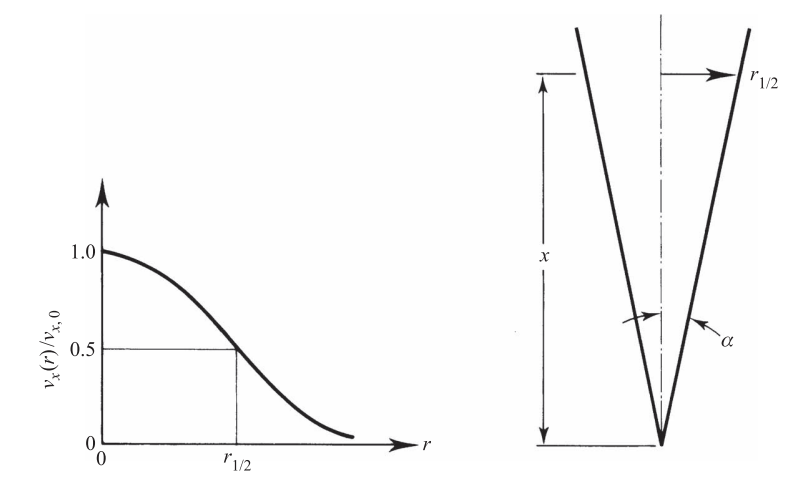
\includegraphics[width=.3\textwidth]{img/spreading_laminar.png}
\end{figure}

\begin{eqnarray}
    r_{1/2}/x &=& 2.97\left(\frac{\mu}{\rho v_e R}\right)=2.97 Re_j^{-1}\\
    \alpha &\equiv& \arctan(r_{1/2}/x)
\end{eqnarray}

对于浓度场,由于我们有施密特数等于1的假设,所以他无量纲的形式实质上和速度完全相同:
\begin{eqnarray}
    Y_F &=& 0.375 Re_j(x/R)^{-1}(1+\xi^2/4)^{-2}\\
    Y_{F,0} &=& 0.375 Re_j(x/R)^{-1}
\end{eqnarray}

上面这些式子的适用范围为:

\begin{equation}
    x/R > 0.375 Re_j
\end{equation}

\begin{enumerate}
    \item 低速射流的燃料浓度衰减到与高速射流(相差10倍)相同的值时,其轴向距离只是高速射流时的 1/10。
    \item 对于给定的燃料(\(\mu/\rho\) 为常数),燃料质量分数的空间分布只与初始的体积流量有关。
\end{enumerate}

\subsection{射流火焰的物理描述}
在流场中,燃料和氧化剂之比为化学当量的点就构成了火焰面。
对于富氧燃烧,火焰长度\(L_f\)定义为:
\begin{equation}
    \Phi(r=0, x=L_f) = 1.0
\end{equation}

\begin{itemize}
    \item 发生化学反应的区域通常是很窄的,到达顶部以前,高温区域是环状的。
    \item 按说应该考虑浮力,但是考虑到拉长之后,扩散作用也会变强,所以两个可以近似认为是抵消了。
    \item 对于圆口火焰,火焰长度和初始速度及管径都无关,粗略估算:
    \begin{equation}
        L_f\approx \frac{3}{8\pi}\frac{Q_F}{\mathcal{D}Y_\mathrm{F,stoic}}
    \end{equation}火焰长度确实是和\textit{体积流量}成正比,而且还和燃料的化学当量质量分数成反比。
\end{itemize}

\subsection{简化理论描述}

\subsubsection{基本假设}

\begin{enumerate}
    \item 流动为稳定的轴对称层流,燃料由半径为R 的圆形喷嘴喷出,在静止、无限大、充满氧化剂的空间里燃烧。
    \item 火焰内部只有燃料和产物,火焰外部只有产物和氧化剂。
    \item 在火焰表面,燃料和氧化剂按化学当量比进行反应。化学动力学速度无限快,火焰只存在于一个无限薄的薄层里。\textbf{火焰面近似}。
    \item 服从菲克扩散定律的简单二元扩散.
    \item 路易斯数(\(Le=\alpha/\mathcal{D}\)等于1。
    \item 忽略辐换热。
    \item 只考虑径向的动量、热量和物质扩散,而忽略轴向的各种扩散。
    \item 火焰的轴线垂直向上。
\end{enumerate}

\subsubsection{基本守恒方程}
\begin{enumerate}
    \item 质量守恒;
    \begin{equation}
        \frac{1}{r}\frac{\partial(r\rho v_{r})}{\partial r}+\frac{\partial(\rho v_{x})}{\partial x}=0.
    \end{equation}
    \item 轴向动量守恒;
    \begin{equation}
        \frac{1}{r}\frac{\partial}{\partial x}(r\rho v_{x}v_{x})+\frac{1}{r}\frac{\partial}{\partial r}(r\rho v_{x}v_{r})-\frac{1}{r}\frac{\partial}{\partial r}\!\left(r\mu\frac{\partial v_{x}}{\partial r}\right)=(\rho_{\infty}-\rho)g.
    \end{equation}
    \item 组份守恒:燃料一个、氧化剂一个,然后直接算出产物;
    \begin{equation}
        \frac{1}{r}\frac{\partial}{\partial x}(r\rho v_{x}Y_{i})+\frac{1}{r}\frac{\partial}{\partial r}(r\rho v_{r}Y_{i})-\frac{1}{r}\frac{\partial}{\partial r}\biggl(r\rho D\frac{\partial Y_{i}}{\partial r}\biggr)=0,
    \end{equation}
    \begin{equation}
        Y_{Pr} = 1 - Y_F - Y_{Ox}
    \end{equation}
    \item 能量守恒:Shvab-Zeldovich形式。式子在火焰面内、外都适用,但是在火焰面处不连续。反应放出的热量必将以边界条件的形式给出。在这里,边界指的是火焰面。
{\tiny
        \begin{equation}
        \frac{\pp}{\pp x}\left(r\rho v_x \int c_p \dd T\right) + \frac{\pp}{\pp r}\left(r \rho v_r \int c_p \dd T\right) - \frac{\pp}{\pp r}\left(r\rho \mathcal{D} \frac{\pp \int c_p \dd T}{\pp r}\right) = 0
    \end{equation}}
\end{enumerate}

\subsubsection{附加关系式}
状态方程:

\begin{equation}
    \rho = \frac{P MW_\mathrm{mix}}{R_u T}
\end{equation}

\begin{equation}
    MW_\mathrm{mix} = \left(\sum Y_i / MW_i\right)^{-1}
\end{equation}

这些是偏微分方程,而且我们还不知道火焰面的位置,不好弄,我们要考虑守恒标量。

\subsubsection{守恒标量的推导}

\begin{enumerate}
    \item 混合物分数;
    \[
        f = Y_F + \left(\frac{1}{\nu + 1}\right)Y_{Pr}
    \]
    实际求解完之后,只需要找到\(f=f_\mathrm{stoic}\)的位置,就能确定火焰面的位置。\(f_\mathrm{stoic} = \frac{1}{\nu+1}\).
    \item 标准焓;
    \item 无量纲方程:无量纲轴向距离、无量纲径向距离、无量纲轴向速度、无量纲径向速度、无量纲标准焓、无量纲密度。基于这些变量可以写出无量纲的连续性、轴向动量、混合物分数、无量纲焓的方程和对应的边界条件。具体内容看书271。

    其中,混合物分数和无量纲焓的方程及边界条件是完全相同的,那么我们其实解一个就可以了。
    \item 附加假设:认为施密特数\(Sc=\mu/\rho \mathcal{D}\)等于1,那么这样的话:轴向动量、混合物分数、焓方程都统一了。
    {\tiny\begin{equation}
        \frac{\pp}{\pp x^*}(r^* \rho^* v_x^*\xi)+\frac{\pp}{\pp r^*}(r^* \rho^* v_x^*\xi) - \frac{\pp}{\pp r^*}\left(\frac{1}{Re}r^*\frac{\pp \xi}{\pp r^*}\right)=0
    \end{equation}}
    这里面的\(\xi = v_x^*=f=h^*\),雷诺数\(Re=\rho_e v_e R/\mu\)。

    当然,速度和密度还需要满足连续性方程,密度和焓还需要满足状态关系式
    \item 状态关系式。
\end{enumerate}

进行最后的一些简化:
\begin{itemize}
    \item 各组分的比热容均为常数。
    \item 氧化剂和产物的生成焙均为零:燃料的生成熔和燃烧热相等。
\end{itemize}

\subsubsection{各种不同的解法}

\subsection{圆口和槽型口燃烧器的火焰长度}
\subsubsection{罗帕关联式}

对于圆口和方口燃烧器,可以用下面的表达式来计算火焰长度。这些结果适用于富氧燃烧的情况,而不管燃烧中动力因素和浮力因素哪个占的地位更重,也不管燃料喷射进入的是静止的氧化剂空间还是和燃料氧化剂同轴射流。

\begin{enumerate}
    \item 圆口:
    \begin{equation}
        \begin{aligned}
            L_\mathrm{f,thy} &= \frac{Q_F(T_\infty / T_F)}{4\pi \mathcal{D}_\infty \ln(1+1/S)}\left(\frac{T_\infty}{T_f}\right)^{0.67}\\
            L_\mathrm{f,expt} &= 1330\frac{Q_F (T_\infty/T_F)}{\ln(1+1/S)}
        \end{aligned}
    \end{equation}
    其中\(S\)是化学当量氧化剂-燃料摩尔比;\(\mathcal{D}_\infty\)是氧化剂的平均扩散系数;F代表燃料,f代表火焰。注意,在这个式子中并没有出现\textit{燃烧器直径}。
    \item 方口:
    \begin{equation}
        \begin{aligned}
        {L}_{f,\mathrm{thy}}&=\frac{Q_{F}(T_{\infty}/T_{F})}{16\mathcal{D}_{\infty}\left[\mathrm{inverf}((1+S)^{-0.5})\right]^{2}}\left(\frac{T_{\infty}}{T_{f}}\right)^{0.67}\\
        L_{f,\mathrm{expt}}&=1045\,{\frac{Q_{F}(T_{\infty}/T_{F})}{[\mathrm{inverf}((1+S)^{-0.5})]^{2}}},\\
        \end{aligned}
    \end{equation}
    \item 槽形口-浮力控制:浮力的作用通过平均浮力加速度来估计,\(a\approx 0.6 g(T_f/T_\infty -1)\),在\(T_f=1500\)K 时,火焰长度和\(a\)的-1/3次方成正比。
    \item 槽形口-过渡区控制;
\end{enumerate}

流动为何种控制利用下面的标准来判断:
\begin{enumerate}
    \item \(Fr_f\gg 1\):动量控制;
    \item \(Fr_f\approx 1\):混合(过渡区);
    \item \(Fr_f\ll 1\):浮力控制。
\end{enumerate}

\subsubsection{流量和几何形状的影响}
\begin{multicols}{2}
    \begin{figure}[H]
        \centering
        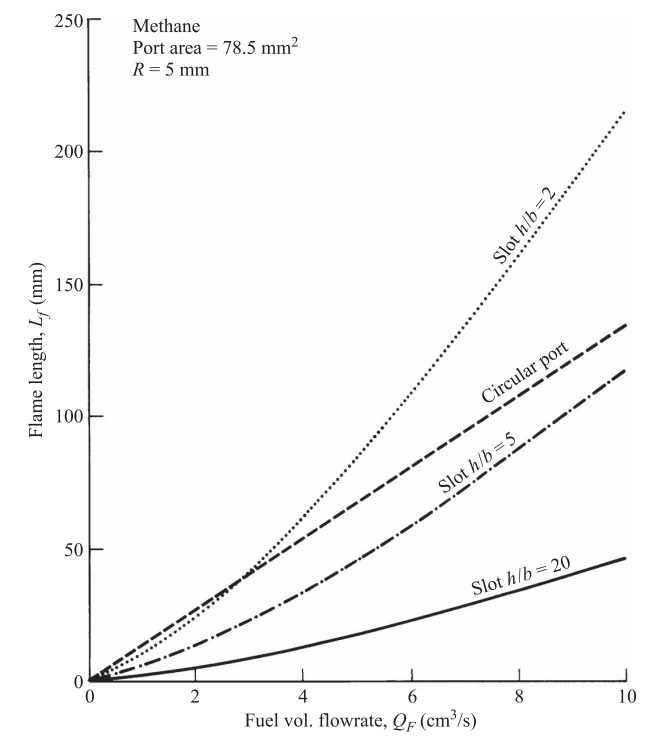
\includegraphics[width=.15\textwidth]{img/laminar_length.png}
    \end{figure}
    {
        \tiny
        出口面积相等,出口平均速度相等,\(Fr\)很小,受浮力控制。
        \begin{enumerate}
            \item 圆口燃烧器的火焰长度和燃料的体积流率呈线性关系;
            \item 槽形口的火焰程度对燃料体积流量的变化率比线性更强;
            \item 槽形口燃烧起喷口变窄,火焰也会变短。
        \end{enumerate}
    }
\end{multicols}

\subsubsection{影响化学当量的因素}

\begin{equation}
    S = \left(\frac{\text{moles ambiet fluid}}{\text{modles nozzle fluid}}\right)_\text{stoic}.
\end{equation}

\begin{enumerate}
    \item 燃料类型:\(S = (x+y/4)/(\chi_\mathrm{O_2})\)。碳氢比越高,火焰长度越长,高碳烃之间大家大差不差。
    \item 一次风:\(S = (1-\psi_\text{pri})/(\psi_\text{pri}+(1/S_\text{pure}))\)。\(\psi_\text{pri}\)是一次风量占所需空气的百分比,即一次风率;\(S_\text{pure}\)是纯燃料对应的化学当量摩尔比。引入一次风,火焰长度变短,防止碳烟形成。
    \item 氧化剂的含氧量:含氧量越高,火焰长度越短。以甲烷在纯氧中和空气中燃烧为例,前者的火焰长度只有后者的四分之一左右。有两幅图可以看看284.
    \item 燃料中加入惰性气体来稀释:\(S = (x+y/4)/(\chi_\mathrm{O_2}/(1-\chi_\text{dil}))\)
\end{enumerate}

\subsection{碳烟的形成和分解}

\begin{enumerate}
    \item 前体物的形成:多环芳烃(PAH)与乙炔反应长大;
    \item 开始形成颗粒:形成临界尺寸(3000~10000原子质量单位)的小颗粒;
    \item 颗粒的长大和聚合;
    \item 颗粒被氧化。
    \item 碳烟总是在火焰下的反应区内形成,并且其流动的流线在接近焰舌时才能和反应区相交。
\end{enumerate}

\textbf{发烟点}:逐渐增大燃料的流量,直到焰舌处开始出现烟为止。